\documentclass[pageno]{cos429}

\newcommand{\quotes}[1]{``#1''}

\widowpenalty=9999

\usepackage[normalem]{ulem}
\usepackage{amsmath}
\usepackage{algorithm2e}
\usepackage{subfig}

\DeclareMathOperator*{\argmin}{arg\,min}
\DeclareMathOperator*{\image_label}{label}

\begin{document}

\title{Robustness of Face Recognition to Image Manipulations}

\author{Cathy Chen (cc27), Zachary Liu (zsliu), and Lindy Zeng (lindy)}
\date{}
\maketitle

\section{Motivation}
We can often recognize pictures of people we know even if the image has low resolution or obscures part of the face, if the camera angle resulted in a distorted image of the subject's face, or if the subject has aged or put on makeup since we last saw them. Although this is a simple recognition task for a human, when we think about how we accomplish this task, it seems non-trivial for computer algorithms to recognize faces despite visual changes.

Computer facial recognition is relied upon for many application where accuracy is important. Facial recognition systems have applications ranging from airport security and suspect identification to personal device authentication and face tagging \cite{huang_face_2011}. In these real-world applications, the system must continue to recognize images of a person who looks slightly different due to the passage of time, a change in environment, or a difference in clothing.

Therefore, we are interested in investigating face recognition algorithms and their robustness to image changes resulting from realistically plausible manipulations. Furthermore, we are curious about whether the impact of image manipulations on computer algorithms' face recognition ability mirrors related insights from neuroscience about humans' face recognition abilities.

\section{Goal}
In this project, we implement both face recognition algorithms and image manipulations. We then analyze the impact of each image manipulation on the recognition accuracy each algorithm, and how these influences depend on the accuracy of each algorithm on non-manipulated images.

\section{Background and Related Work}
Researchers have developed a wide variety of face recognition algorithms, such as traditional statistical methods such as PCA, more opaque methods such as deep neural networks, and proprietary systems used by governments and corporations \cite{noauthor_face_nodate}\cite{schroff_facenet:_2015}\cite{sun_meet_2017}.

Similarly, others have developed image manipulations using principles from linear algebra, such as mimicking distortions from lens distortions, as well as using neural networks, such as a system for transforming images according to specified characteristics \cite{savarese_camera_2015}\cite{upchurch_deep_2016}.

Furthermore, researchers in psychology have studied face recognition in humans. A study of "super-recognizers" (people with extraordinarily high powers of face recognition) and "developmental prosopagnosics" (people with severely impaired face recognition abilities) found that inverting images of faces impaired recognition ability more for people with stronger face recognition abilities \cite{russell_super-recognizers:_2009}. This could indicate that image manipulations tend to equalize face recognition abilities, and we investigate whether this is the case with the manipulations and face recognition algorithms we test.

\section{Methods}
To test robustness of image recognition algorithms, we implement various algorithms and image manipulations. We then test each of the algorithms with un-manipulated images as well as images resulting from each of the manipulations. In addition to the absolute accuracy of each of these combinations, we analyze the trend in each algorithm's performance on manipulated images to the algorithm's performance on un-manipulated images.

We describe our algorithms, manipulations, dataset, and evaluation method in the following subsections.

Our implementation is available online, as further described in the Appendix (\ref{sec:Appendix}).

\subsection{Algorithms}
\subsubsection{PCA}\hspace*{\fill} \\
We implement this algorithm according to details described in \cite{vidal_eigenfaces_2008}, based on the work of \cite{turk_eigenfaces_1991}.

We first find the principal components of the training images, and we call these principal components "eigenfaces". To classify a face, we then project the face into the space spanned by these eigenfaces and project each training face image to the same subspace. We classify the test face according to the label of the closest projected training face, where we define closeness by the Frobenius norm of the difference between the test face and each training face.

So the algorithm performs face recognition by solving $\image_label(\argmin||\Omega-\Omega_i||_2)$ where $\Omega$ is the coordinates of the test image in eigenface space and $\Omega_i$ is the coordinates of training image $i$ in eigenface space.

\subsubsection{Sparse Representation}\label{sec:sparse_representation}\hspace*{\fill} \\
We implement this algorithm according to the descriptions found in \cite{ganesh_face_2012}.

To classify a face, we first encode it as a sparse representation of the training faces. We then classify the test face according to the label whose training faces receive the greatest weight in this sparse representation.

So the algorithm performs face recognition by solving $\min||c||_1\:s.t.\:||y-\Phi c||\leq\epsilon$ and then choosing the label with the greatest weights in $c$, where $\Phi$ is the training images and $y$ is the test image.

\subsubsection{Sparse Representation with Dimension Reduction}\hspace*{\fill} \\
We implement this algorithm according to the descriptions found in \cite{ganesh_face_2012}.

We first project the test and training faces to a lower-dimension subspace using PCA, and then proceed with face classification according to the method described in section \ref{sec:sparse_representation}.
\subsubsection{Sparse Representation with Combined L1 Loss}\hspace*{\fill} \\
We implement this algorithm according to the descriptions found in \cite{ganesh_face_2012}.

We first project the test and training faces to a lower-dimension subspace using PCA, and then find a sparse encoding of the test face using a dictionary with the projected training faces in addition to the standard basis vectors. Using this sparse encoding, we perform classification as described in section \ref{sec:sparse_representation}.

So this algorithm performs face recognition by solving $\min||c||_1+||e||_1\:s.t.\:y=\Phi c+e$, where the addition of $e$ is intended to allow the algorithm to account for small differences between images of the same person.

\subsection{Support Vector Machine (SVM)}
While we did not implement this algorithm, we include results from this algorithm as an additional comparison point. We use the stock support vector machine classifier implementation provided in the scikit-learn Python library. We use the default parameters, including the use of an RBF kernel \cite{scikit-learn}.

\subsubsection{VGG-based Classification}\hspace*{\fill} \\
We implement this algorithm based on the work and pre-trained convolutional neural network of \cite{parkhi_deep_2015}. Each image undergoes preprocessing before usage in the network. For the preprocessing, we use the deformable parts model face detector provided by \cite{parkhi_deep_2015} and crop the detected face from each of the the original images. An example of a face before and after preprocessing is shown in Figure \ref{fig:vgg_preprocessing}. We also subtract the mean values for each color channel, provided by \cite{parkhi_deep_2015}, from the images prior to using the convolutional neural network.

\begin{figure}[!htb]
\subfloat[Original Image]{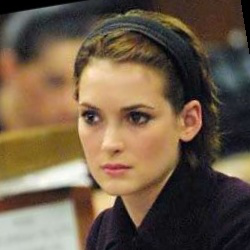
\includegraphics[width = 3in]{../figures/vgg_2.png}}
\subfloat[Preprocessed Image]{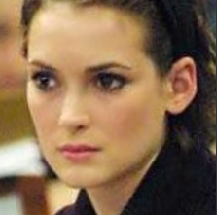
\includegraphics[width = 3in]{../figures/vgg_3.png}}
\caption{Preprocessing Demo (The face is detected and cropped from the original image).}
\label{fig:vgg_preprocessing}

\end{figure}

Next, we translate the architecture of the VGG-FACE network for use with the Keras Python framework and load the pre-trained weights. We feed each face through the network, stopping at the fc-7 layer to obtain a 4,096-dimensional descriptor for each image.

For each test descriptor $w$, we calculate its cosine similarity to each training descriptor $v$. This is given by $arccos\frac{v \cdot w}{||v|| ||w||}$. The use of cosine similarity is different from the Euclidean distance methodology used in \cite{parkhi_deep_2015}, which we found to have weaker performance on our dataset. We find the nearest-$k$ neighboring training descriptors according to cosine similarity and classify the test face according to the majority vote.

\subsection{Image Manipulations}

\subsubsection{Occlusion}\hspace*{\fill} \\
The tendency for external objects to hide parts of people's faces in images motivates this manipulation. For instance, a large hat or physically faded spots on an image could hide part of someone's face, but we should still recognize the image as the same person.

We implement occlusion by selecting a region of the image and randomly resetting the pixels in this region, and show examples of occluded images in Figure \ref{fig:manipulationdemo_occlusion}. We vary the occlusion window size to produce dataset images with varying amounts of occlusion.

\begin{figure}[!htb]
\subfloat[Original Image]{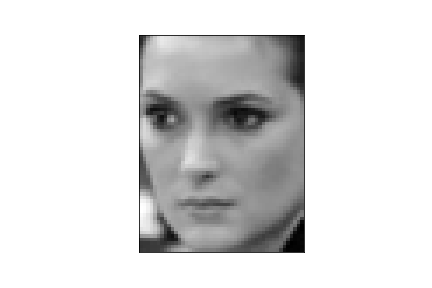
\includegraphics[width = 3in]{../figures/manipulationdemo_none}}
\subfloat[Occluded Image]{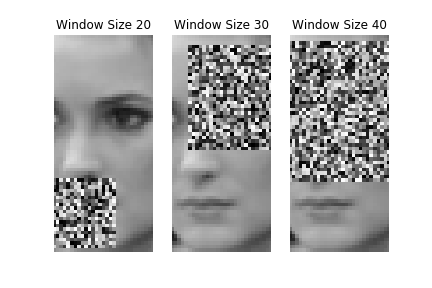
\includegraphics[width = 3in]{../figures/manipulationdemo_occlusion}}
\caption{Occlusion Demo (Window size is length of occluded region on one size).}
\label{fig:manipulationdemo_occlusion}
\end{figure}

\subsubsection{Radial Distortion}\hspace*{\fill} \\
Distortions caused by camera lenses motivate these manipulations. In particular, spherical camera lenses cause two types of radial distortion: barrel distortion disproportionately magnifies pixels closer to the optical axis and can occur with smaller focal length lenses, while pincushion distortion disproportionately magnifies pixels farther from the optical axis and can occur with larger focal length lenses \cite{drap_exact_2016}.

We mimic barrel distortion according to descriptions found in \cite{gribbon_real-time_2003}, and adapt this method for pincushion distortion as described in \cite{drap_exact_2016}.

We set $(i_0,j_0)$ as the vertical and horizontal centerline of the image, and replace the pixel at $(i,j)$ with the pixel at $(\frac{i}{1+kr^2},\frac{j}{1+kr^2})$ where $r=\sqrt{(i-i_0)^2+(j-j_0)^2}$ and $k$ is a selected parameter. A positive $k$ results in barrel distortion, while a negative $k$ results in pincushion distortion.

We provide examples of pincushion and barrel distortion for various values of $k$ in Figure \ref{fig:manipulationdemo_radial}. We manipulate our dataset images with various levels of radial distortion, as determined by $k$.

\begin{figure}[!htb]
\subfloat[Original Image]{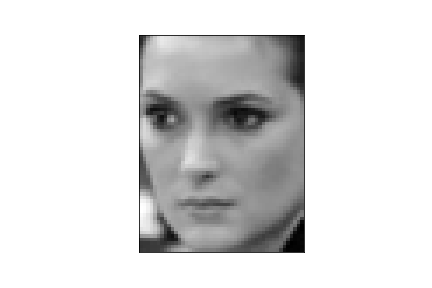
\includegraphics[width = 3in]{../figures/manipulationdemo_none}}
\subfloat[Distorted Image]{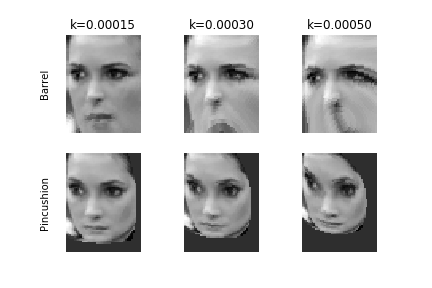
\includegraphics[width = 3in]{../figures/manipulationdemo_radial}}
\caption{Radial Distortion Demo.}
\label{fig:manipulationdemo_radial}
\end{figure}

\subsubsection{Blur}\hspace*{\fill} \\
The possibility for image recognition systems to receive blurry input motivates this manipulation. We mimic blurry images by replacing each pixel by the mean value of the pixels within a pre-specified window of the replaced pixel. We manipulate our dataset images with various levels of blur.

We provide examples of blurred images in Figure \ref{fig:manipulationdemo_blur}.
\begin{figure}[!htb]
\subfloat[Original Image]{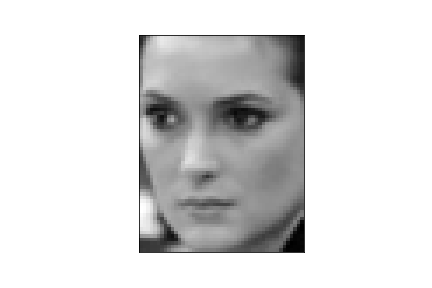
\includegraphics[width = 3in]{../figures/manipulationdemo_none}}
\subfloat[Blurred Image]{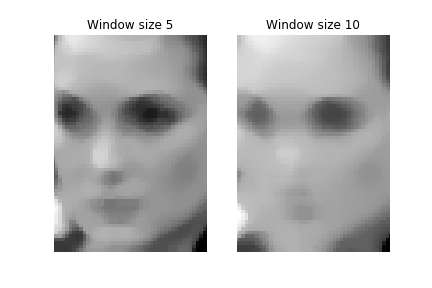
\includegraphics[width = 3in]{../figures/manipulationdemo_blur}}
\caption{Blur Distortion Demo (Window size is length of window of pixels whose mean replaces each original pixel).}
\label{fig:manipulationdemo_blur}
\end{figure}

\subsection{Deep Feature Interpolation}\hspace*{\fill} \\
We apply the Deep Feature Interpolation (DFI) algorithm based on the work and implementation of \cite{upchurch_deep_2016}. This algorithm provides a framework for performing content editing of a facial image. It works by interpolating between attributes in the feature space of a deep convolutional neural network, specifically the VGG network.

DFI is a versatile algorithm which can, for example, make a face look older or add a moustache to a face, as well as many other possibilities. To make a face look older, it is necessary to find a attribute vector that provides a mapping from a ``younger'' image to an ``older'' image. Thus, for each target attribute (``senior'', ``moustache'', etc.) it is necessary to identify a corresponding source attribute (i.e. ``young'', ``no facial hair'').

Given an input image, and a source-target attribute pair, the algorithm applies the following steps:

\begin{enumerate}
    \item Identify a set of $k$ images in the image dataset which have the source attribute and which are most similar to the input image. Various definitions of similarity are possible. In the implementation we used, similarity is defined by filtering on gender and ranking images based on the number of matching attributes.
    \item Identify a set of $k$ images which have the target attribute in the same manner.
    \item Map these images to VGG feature space and compute the mean vector of each set.
    \item Subtract the mean vectors to compute the attribute vector $w$.
    \item Transform the input image into feature space, and add $\alpha w$, where $\alpha$ is an interpolation parameter.
    \item Perform an inverse mapping back into color space by applying the gradient descent method of \cite{DBLP:journals/corr/MahendranV14}.
\end{enumerate}

We adapt a sample implementation of this algorithm for our implementation, keeping the original parameter values of $k = 1$ and $\alpha = 0.4$.

Figure \ref{fig:dfi} demonstrates the results of this algorithm on one image from the dataset. In our experiments, we use DFI to apply two manipulations: ``senior'' to make the face look older, and ``moustache'' to add a moustache to the face.

\begin{figure}
    \centering
    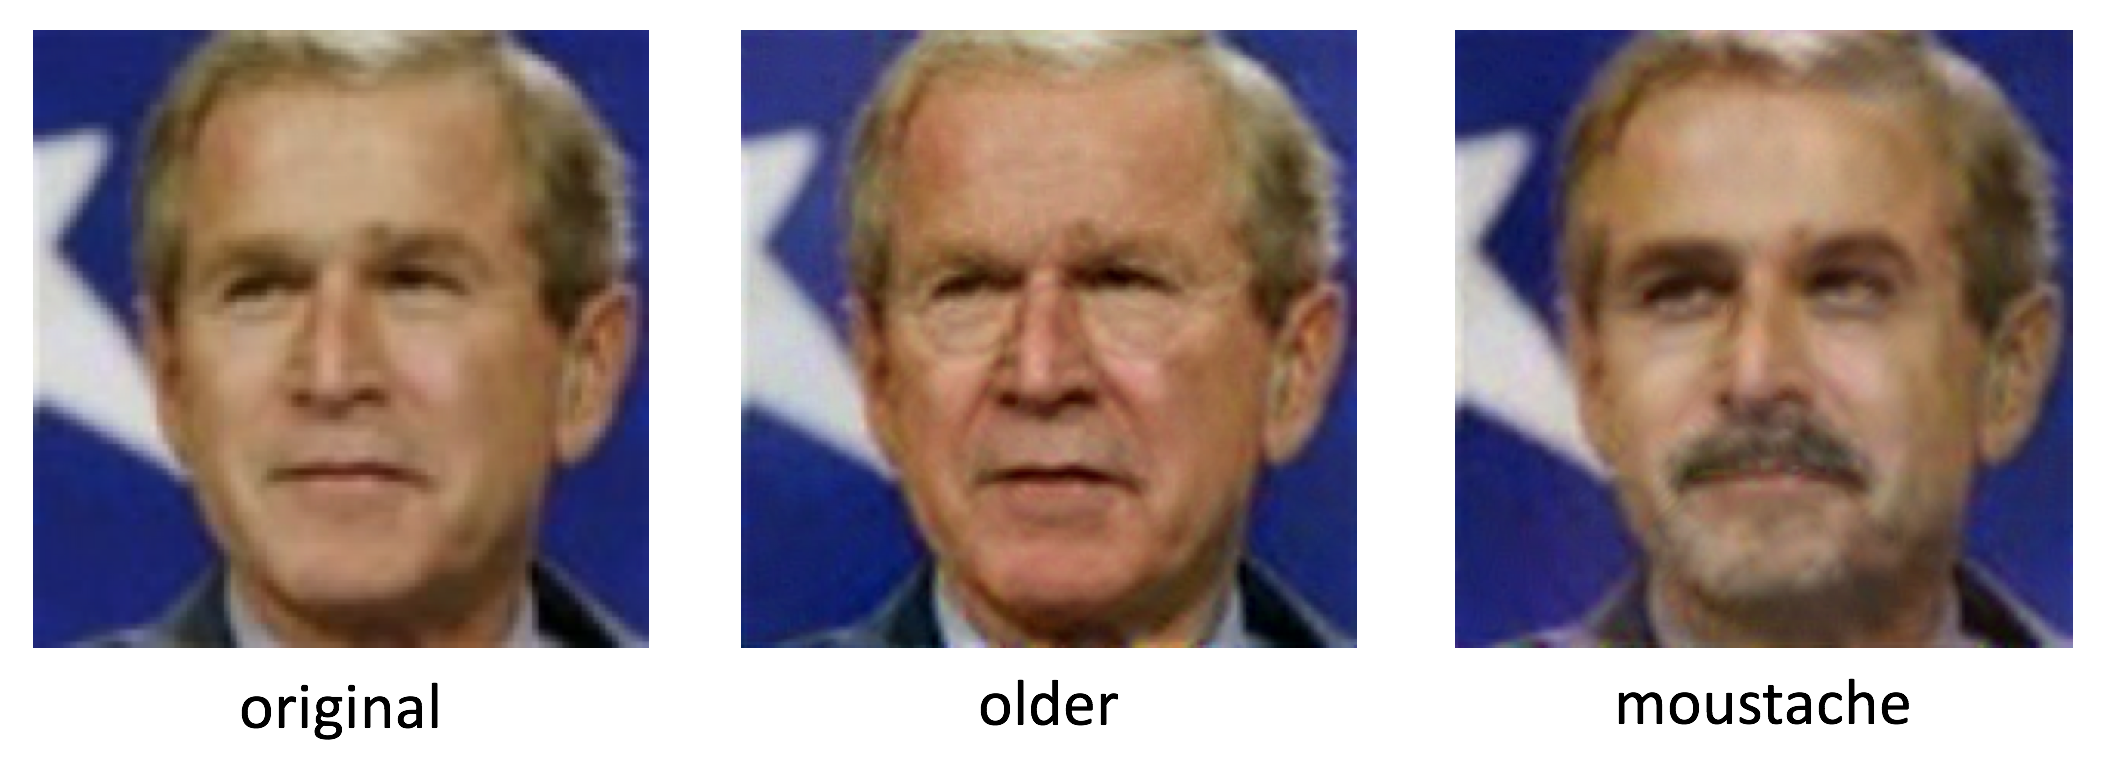
\includegraphics[width=0.6\textwidth]{../figures/dfi.png}
    \caption{DFI output sample with two manipulation types.}
    \label{fig:dfi}
\end{figure}

\subsection{Dataset}\label{sec:data}
We use the Labeled Faces in the Wild Dataset (LFW) \cite{huang_labeled_2007}. We chose this dataset because it contains many ($13,000$) labeled images of different people ($1,680$ of whom have at least two distinct images and $62$ of whom have at least twenty distinct images). This provides sufficient training data for our experiments.

Furthermore, each of image is centered on a single face, which provides some measure of standardization between (non-manipulated) images. This allows us to control the amount and type of manipulation which we then add in our experiments, which is important because we test the robustness of algorithms to specific manipulations.

To improve the accuracy of the recognition algorithms, we use an aligned version of the dataset provided by the DFI implementation. This version of the dataset was aligned using a deep neural network and has better alignment than the ``funneled'' versions of the LFW dataset \cite{noauthor_lfw_nodate}.

\subsection{Evaluation}
We train each algorithm using three instances of each person's face. We then evaluate each algorithm's performance according to its accuracy ($\frac{\textrm{correct predictions}}{\textrm{total predictions}}$) in recognizing faces on the test set, which includes the remaining instances of each person's face.

\section{Results and Discussion}
\subsection*{Baseline Performance}
Our baseline test accuracy with no manipulations on the LFW images is shown in Figure \ref{fig:baseline}. We vary the number of training faces used per person and calculate the accuracy for each algorithm. These baseline results indicate that VGG-FACE outperforms PCA, Sparse Representation, and SVM methods with both 3 and 15 training faces per person. In the interest of computation cost, we did not test the performance of VGG-FACE on the 10 and 19 training faces per person.

\begin{figure}
\centering
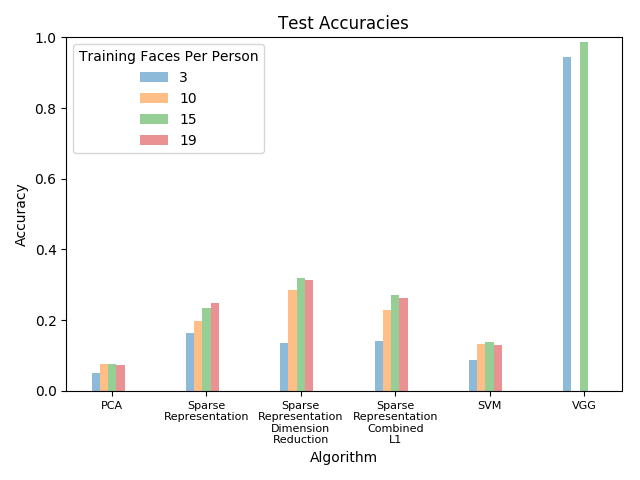
\includegraphics[scale=0.5]{../figures/results_plots/default_accuracies_difftraintest.png}
\caption{Baseline results with no manipulation.}
\label{fig:baseline}
\end{figure}

Further adjustments were made to the VGG-FACE network that produced varying results; the highest accuracy achieved was over 0.98 on non-manipulated images for various values of $k$, where $k$ is the number of nearest neighboring training descriptors to compare to for each test image. We found that preprocessing the images through face detection and cropping improved performance. In addition, using cosine similarity and the nearest-$k$ neighboring heuristic, instead of Euclidean distance and the mean of the training descriptors, also improved performance. We show a summary of the VGG-FACE network's performance on non-manipulated images of the LFW dataset in Figure \ref{fig:vgg_nonmanipulated}.

\begin{figure}
\centering
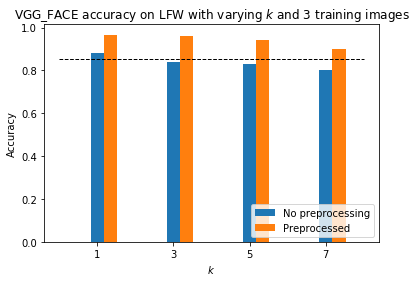
\includegraphics[scale=0.5]{../figures/results_plots/vgg_1.png}
\caption{VGG-FACE Results with No Manipulations (The dotted line indicates performance with Euclidean distance and mean descriptor).}
\label{fig:vgg_nonmanipulated}
\end{figure}

\subsection*{Performance on Manipulated Images}
With manipulations, we find support for image manipulations equalizing face recognition ability. Figure \ref{fig:results_all} shows test accuracies for each algorithm for each type of image manipulation, using 15 images per face to train. As images are occluded by increasing areas, more blurred, or more radially distorted, the test accuracies drop for each algorithm. With the exception of the VGG-FACE algorithm a higher baseline accuracy corresponds to a greater drop in performance on manipulated images, as shown in the left of Figure \ref{fig:results_diff}.

Figure \ref{fig:results_algorithms} shows the results split by algorithm in order to compare the effects of different manipulations. We observe that in 5 out of the 6 algorithms, accuracy drops severely after applying an occlusion manipulation. Only the VGG model is able to handle occlusions well, and it is able to maintain close to baseline accuracy for small occlusions.

However, Figure \ref{fig:results_algorithms} also shows that the DFI manipulations had a relatively small impact on the accuracy of statistical methods, while it had the greatest impact on the VGG model. This shows that the statistical models have better ability to generalize the identity of a face to be robust to these types of content-based manipulations.

In order to compare the change in accuracy across manipulation parameters and different algorithms, we normalize the difference with the baseline accuracies, as shown in the right of Figure \ref{fig:results_diff}. The normalized differences indicate that image manipulations does not clearly impair face recognition accuracy more for algorithms that perform better at baseline.

\begin{figure}[ht]
\centering
\subfloat{
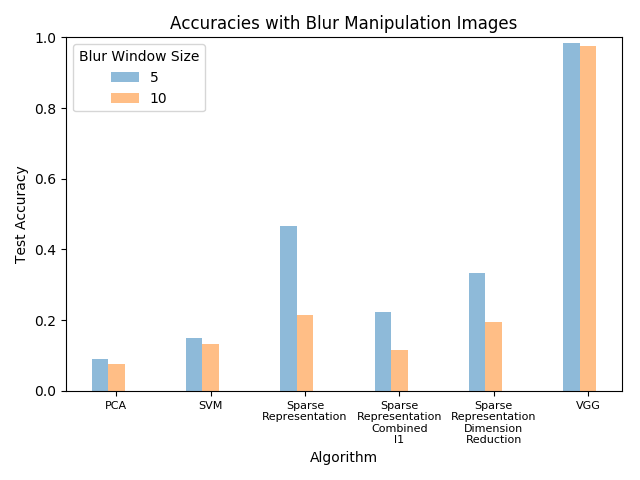
\includegraphics[width=0.5\textwidth]{../figures/results_plots/results_blur_15.png}}
\subfloat{
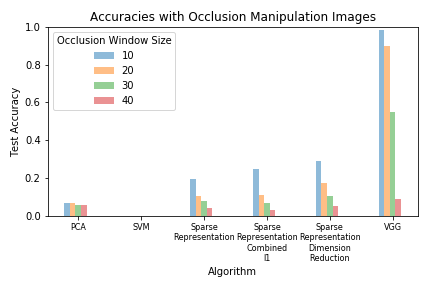
\includegraphics[width=0.5\textwidth]{../figures/results_plots/results_occlude_lfw_15.png}}
\qquad
\subfloat{
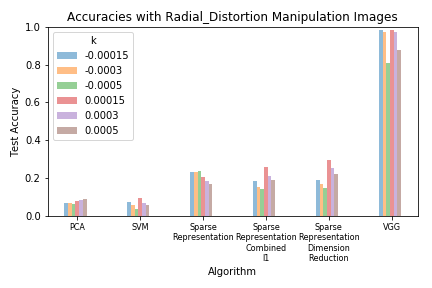
\includegraphics[width=0.5\textwidth]{../figures/results_plots/results_radial_distortion_15.png}}
\subfloat{
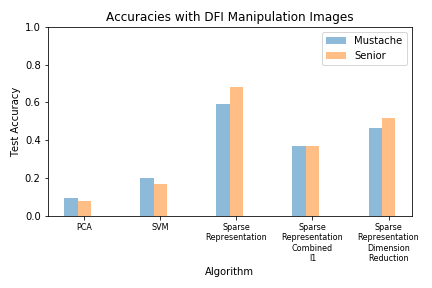
\includegraphics[width=0.5\textwidth]{../figures/results_plots/results_dfi_15.png}}
\caption{Test accuracy across all algorithms and image manipulations for 15 training images.}
\label{fig:results_all}
\end{figure}

\begin{figure}[ht]
    \centering
    \subfloat{
        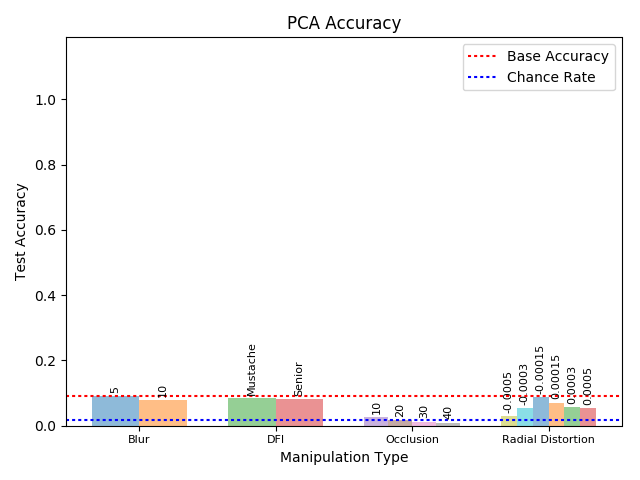
\includegraphics[width=0.5\textwidth]{../figures/results_plots/results_algorithm_PCA_15.png}}
    \subfloat{
        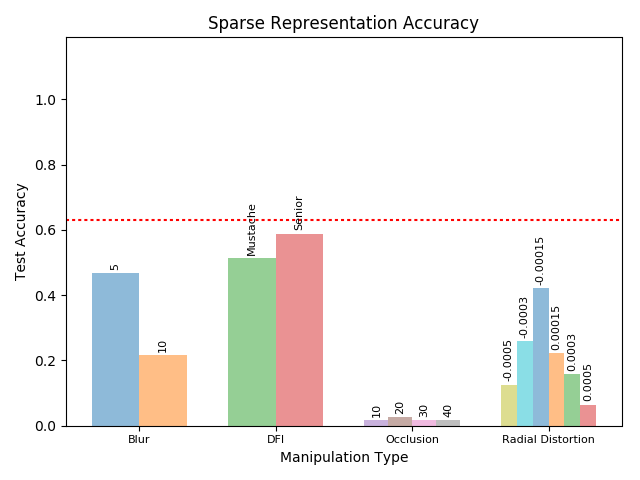
\includegraphics[width=0.5\textwidth]{../figures/results_plots/results_algorithm_SparseRepresentation_15.png}}
    \qquad
    \subfloat{
        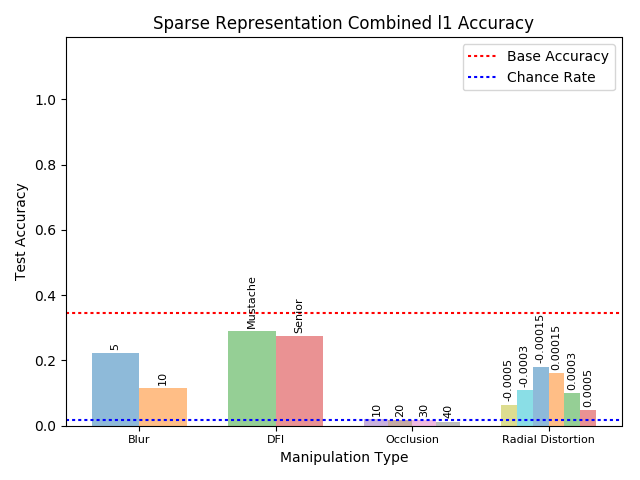
\includegraphics[width=0.5\textwidth]{../figures/results_plots/results_algorithm_SparseRepresentationCombinedl1_15.png}}
    \subfloat{
        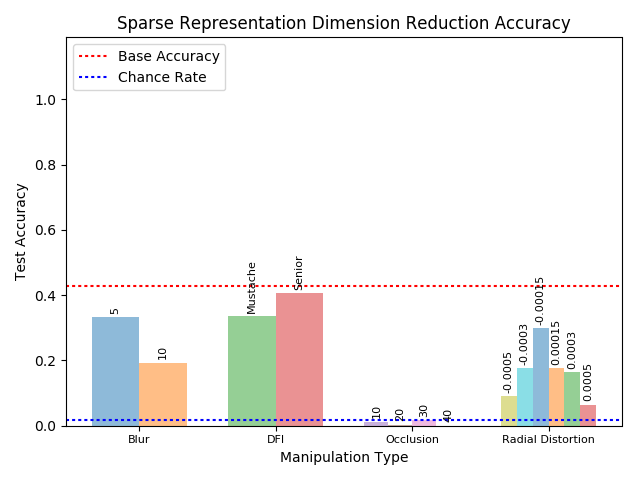
\includegraphics[width=0.5\textwidth]{../figures/results_plots/results_algorithm_SparseRepresentationDimensionReduction_15.png}}
    \qquad
    \subfloat{
        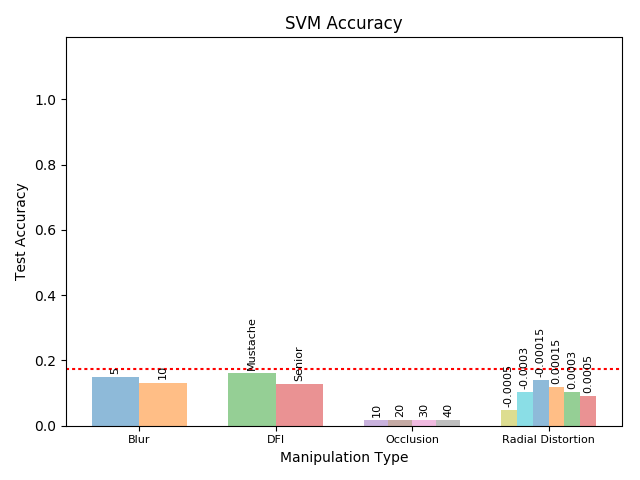
\includegraphics[width=0.5\textwidth]{../figures/results_plots/results_algorithm_SVM_15.png}}
    \subfloat{
        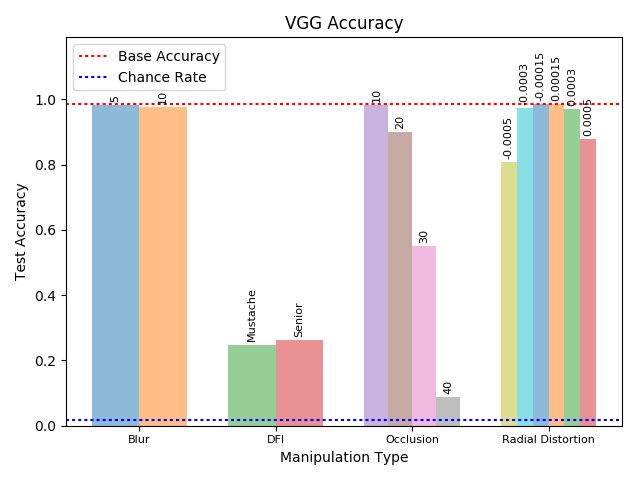
\includegraphics[width=0.5\textwidth]{../figures/results_plots/results_algorithm_VGG_15.png}}
    \caption{Test accuracy (using 15 training examples per face) for each algorithm compared across manipulations. Labels above each bar indicate the corresponding manipulation parameter value used in that experiment.}
    \label{fig:results_algorithms}
\end{figure}

\begin{figure}[ht]
\centering
\subfloat{
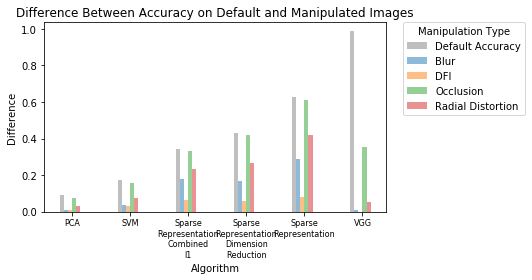
\includegraphics[width=0.5\textwidth]{../figures/results_plots/manipulation_impact_difference.png}}
\subfloat{
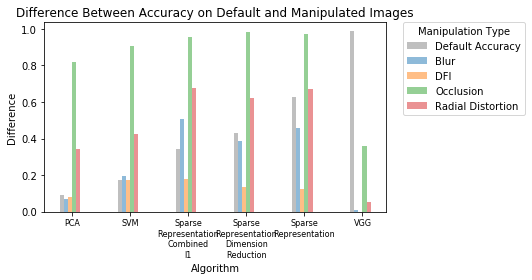
\includegraphics[width=0.5\textwidth]{../figures/results_plots/manipulation_impact_normalizeddifference.png}}
\caption{Absolute difference (left) and normalized difference (right) between test accuracies of different algorithms.}
\label{fig:results_diff}
\end{figure}

\subsection*{Algorithm Strengths and Weaknesses}
With both manipulated and un-manipulated images, VGG far outperforms the other algorithms in terms of recognition accuracy, and this effect is especially pronounced on occluded images. We believe that our statistical algorithms perform especially badly on occluded images because they work by comparing pixel similarities between images -- while DFI, radial distortion, and blur somewhat preserve the pixels themselves, in occluded images a large portion of the image's pixel values are completely lost to the algorithm.

However, a major weakness of VGG is its computational cost. Training VGG on $930$ un-manipulated images took around $42$ minutes, and subsequently testing it on $2093$ test faces took around $12$ minutes. For reference, all of the other algorithms together took $11$ seconds to train and less than $3$ minutes to test on the same dataset.

Another weakness of the system is sensitivity to the alignment of images. With the VGG algorithm, accuracy is lower on the original dataset without face detection and cropping, as shown by the dotted line in Figure \ref{fig:vgg_nonmanipulated}. We mention in Section \ref{sec:data} that the Sparse Representation Algorithms has much better performance on the aligned version of the LFW dataset than the ``funneled'' version. The difference in test accuracies on non-manipulated images between the ``funneled'' and aligned LFW datasets is shown in Figure \ref{fig:results_alignment}. Note that the VGG algorithm used the original ``funneled'' images with additional face detection and cropping.

\begin{figure}[ht]
\centering
\subfloat{
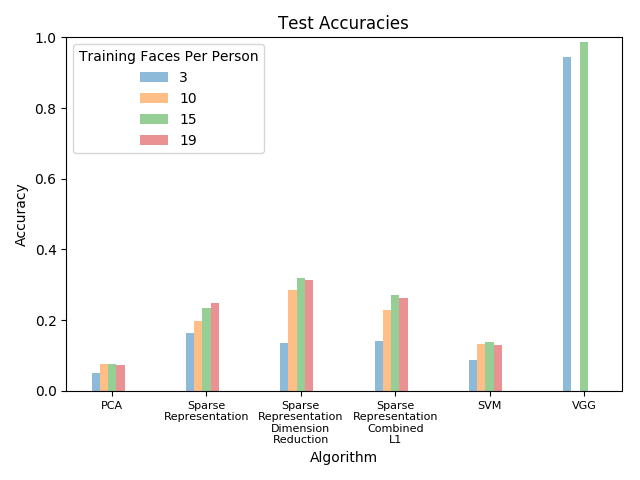
\includegraphics[width=0.5\textwidth]{../figures/results_plots/old_default_accuracies_difftraintest.png}}
\subfloat{
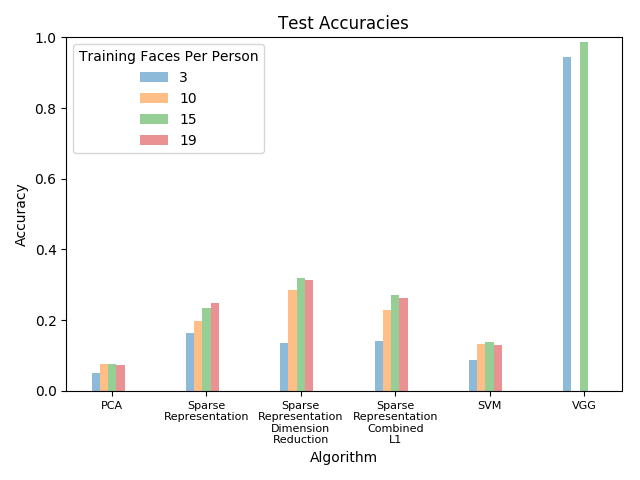
\includegraphics[width=0.5\textwidth]{../figures/results_plots/default_accuracies_difftraintest.png}}
\caption{Results on non-manipulated images for ``funneled'' images (left) and on images for aligned images (right). There is a major improvement in accuracy scores for Sparse Representation algorithms.}
\label{fig:results_alignment}
\end{figure}

\section{Conclusion}
In this project, we implement various face recognition algorithms, ranging from statistical methods such as PCA and Sparse Representation to deep learning methods such as VGG-FACE. We use the Labeled Faces in the Wild dataset, and transform the face images with different manipulations: occlusion, radial distortion, blur, and deep feature interpolation.

When comparing the effects of different face manipulations on different recognition algorithms, we found strengths and weaknesses in the performance of each. Statistical algorithms such as Sparse Representations and SVMs performed well on DFI content-based manipulations, while deep learning methods such as VGG-FACE performed relatively poorly on this manipulation. However, VGG-FACE was able to handle small occlusions, a manipulation which severely impacted the accuracy of statistical models. This shows how each type of recognition model has its own relative strengths, suggesting that a combination of techniques can lead to the highest overall robustness to manipulations.

While VGG-FACE performed the best across non-manipulated and manipulated images, it displayed the same relative accuracy drop as the other algorithms. This suggests that although for humans, people with stronger face recognition ability do worse relatively when identifying manipulated faces, the same cannot be said of stronger and weaker face recognition algorithms.

\bibliographystyle{plain}
\bibliography{cos429bibtex}

\section{Appendix}\label{sec:Appendix}
Our implementation is available \href{https://github.com/cchen23/COS429_final_project}{online}. Our implementation includes a general framework which allows the user to swap in definitions of any image manipulations and recognition algorithms, as well as modules that implement each of the manipulations and algorithms we tested.

\end{document}
